\documentclass{article}
\usepackage[utf8]{inputenc} 
\usepackage[english]{babel}
\usepackage{graphicx}

\title{Marathon of Parallel Programming - 2022\\Problem: k-Nearest Neighbors Classifier}

\author{Kleiton Pereira, Guilherme Piêgas Koslovski} 

\begin{document}

\maketitle 

\section*{Problem definition}

Given a set of two-dimensional points $S$ divided intro $n$ groups, an integer $k$ and a two-dimensional point $P$ to be classified, the k-Nearest Neighbors (KNN) algorithm can be used to solve the classification problem of the point $P$, i.e., classifying the point $P$ into one of the $n$ existing groups based on some criteria.

The KNN algorithm works by comparing the distances from each point $s \in S$ to the point $P$, then selecting the $k$ points with the smallest distance values and counting the frequency of each group in these $k$ points, the point $P$ is then classified to belong to the group with the highest frequency among the $k$ nearest points.

\begin{figure}[h!]
\centering
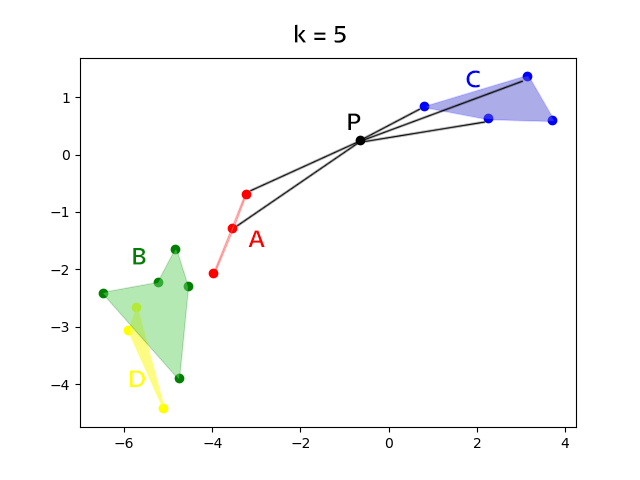
\includegraphics[width=0.8675\textwidth]{input.png}
\caption{Simple example of the KNN classification.}
\label{example}
\end{figure}

The Figure \ref{example} illustrates an example of the KNN classification algorithm being applied. The points have been segregated between 4 different groups (\textit{i.e.}, A, B, C and D) and a point $P$ with no group is provided to be classified, the KNN algorithm then searches for the $k$ points closest to the point $P$ and, after that, the groups have their frequencies counted, with the highest frequency being chosen as the classification of $P$, in the case of this example, the point $P$ is classified to belong to the group C.

\section*{Input}

An input represents the classification of a single point. The first line contains the pattern "n\_groups=$n$", where $n$ is the total number of groups in this input. Then, for each of the $n$ groups the following lines will be provided, the first line has the pattern "label=$c$" where $c$ is a single character that represents the label (\textit{i.e.}, identification) of the group, then the second line follows the pattern "length=$L$", where $L$ is the number of two-dimensional points in this group and then, the next $L$ lines contain the pattern "($x$,$y$)" that represents each point that belongs to the aforementioned group. After all groups have been represented there's a single line with the pattern "k=$k$", where $k$ is the parameter previously discussed. Lastly, the final line also contains the pattern "($x$,$y$)", representing the coordinates to the two-dimensional point to be classified.

\textit{The input must be read form the standard input.}

\section*{Output}

The output contains a single character, it being the label of the group chosen as the classification of the provided point.

\textit{The output must be written to the standard output.}

\section*{Example}

\begin{table}[!ht]
    \begin{tabular}{|p{0.6\linewidth}|c|}
        \hline
        Input example & Output example\\
         & \\
        n\_groups=4 & C\\
        label=A & \\
        length=3 & \\
        (-3.55,-1.28) & \\
        (-3.99,-2.06) & \\
        (-3.23,-0.70) & \\
        label=B & \\
        length=5 & \\
        (-4.85,-1.65) & \\
        (-5.23,-2.22) & \\
        (-4.75,-3.89) & \\
        (-6.48,-2.41) & \\
        (-4.56,-2.29) & \\
        label=C & \\
        length=4 & \\
        (2.25,0.64) & \\
        (0.80,0.85) & \\
        (3.13,1.37) & \\
        (3.71,0.59) & \\
        label=D & \\
        length=3 & \\
        (-5.73,-2.65) & \\
        (-5.11,-4.41) & \\
        (-5.92,-3.06) & \\
        k=5 & \\
        (-0.65,0.25) & \\
         & \\
        \hline
   \end{tabular}
\end{table}

\end{document}

